%! TeX program = lualatex
\documentclass[12pt,a4paper]{article}

\usepackage[nil]{babel}
\usepackage{unicode-math}
\usepackage[svgnames]{xcolor}
\usepackage{lmodern}
\usepackage{graphicx}
\usepackage{wrapfig}
\usepackage{float}
\usepackage{parskip}
\usepackage[font=small,labelfont=bf]{caption}

\babelprovide[import=el, main, onchar=ids fonts]{greek} % can also do import=el-polyton
\babelprovide[import, onchar=ids fonts]{english}

\babelfont{rm}
          [Language=Default]{Liberation Sans}
\babelfont[english]{rm}
          [Language=Default]{Liberation Sans}
\babelfont{sf}
          [Language=Default]{Liberation Sans}
\babelfont{tt}
          [Language=Default]{Liberation Sans}

%Enter Title Here
 \title{Project-description-v0.1 \\ LibShare}
\author{\textbf{Ονόματα / ΑΜ / Έτος:} \\ Γρηγόρης Καπαδούκας / 1072484 / 4\textdegree \\ Χρήστος Μπεστητζάνος / 1072615 / 4\textdegree \\ Νικόλαος Αυγέρης / 1067508 / 5\textdegree \\ Περικλής Κοροντζής / 1072563 / 4\textdegree}

\begin{document}

\makeatletter
\begin{center}
	\LARGE{\@title} \\
	\pagebreak
	\begin{LARGE}\@author\end{LARGE} \\
\end{center}
\pagebreak

%Insert Body Here
\section{Περιγραφή:}
\label{Περιγραφή}
Το προς δημιουργία project λογισμικού αποτελεί μια εφαρμογή Peer-2-Peer ενοικίασης βιβλίων. Δηλαδή η εφαρμογή αυτή επιτρέπει χρήστες να νοικιάζουν βιβλία ο ένας από τον άλλο για χρηματική ανταμοιβή, με ενσωματωμένη ασφάλεια έναντι κλοπών. Ο χρήστης σε πρώτο βήμα θα μπορεί να δημιουργεί προσωπικό λογαριασμό στην εφαρμογή, εισάγοντας το προσωπικό του email, ένα username και ένα password. Μετά τη δημιουργία του λογαριασμού του ο χρήστης θα μπορεί να εισέρχεται στην εφαρμογή εισάγοντας τα στοιχεία του. Στην εφαρμογή του δίνονται οι εξής δυνατότητες:

\begin{itemize}
	\item Θα μπορεί να νοικιάσει ένα βιβλίο από άλλους χρήστες της εφαρμογής. Κατά τη λειτουργία αυτή θα εμφανίζεται μια λίστα από διαθέσιμα βιβλία προς ενοικίαση από χρήστες κοντά του (στην ίδια πόλη με αυτόν) που κάνουν συναλλαγές πρόσωπο με πρόσωπο ή από χρήστες που μένουν μακριά αλλά δέχονται ταχυδρομικές συναλλαγές. 

Έτσι αφού διαλέξει ο χρήστης το βιβλίο που θέλει, (υπάρχει και λειτουργία αναζήτησης στη λίστα) του εμφανίζεται η λίστα των χρηστών που προσφέρουν το βιβλίο αυτό για ενοικίαση. Σε αυτή τη λίστα βλέπει ο χρήστης τους τρόπους συναλλαγής που δέχεται κάθε χρήστης (ταχυδρομικώς ή πρόσωπο με πρόσωπο). Αφού επιλέξει έναν μπορεί να του κάνει "Αίτηση ενοικίασης". Έπειτα της αίτησης, ενημερώνεται ο χρήστης-ιδιοκτήτης του βιβλίου και έχει την επιλογή να δεχτεί ή να απορρίψει την αίτηση αυτή.

Αν τη δεχτεί, οι δύο χρήστες βλέπουν τα στοιχεία επικοινωνίας ο ένας του άλλου και αφού λάβει ο ενοικιαστής το βιβλίο ενημερώνουν οι χρήστες την εφαρμογή και χρεώνεται αυτομάτως ο ενοικιαστής ημερήσια, μέχρι το βιβλίο να επιστραφεί στον ιδιοκτήτη. 

Αλλίως αν η αίτηση του ενοικιαστή απορριφθεί, τότε αυτός ενημερώνεται και δεν γίνεται συναλλαγή.

	\item Ο χρήστης θα μπορεί επίσης να κάνει αναζήτηση άλλων χρηστών με βάση το username τους και να δει τα βιβλία που προσφέρουν για ενοικίαση.

	\item Οι χρήστες θα μπορούν έπειτα από μια συναλλαγή να κάνουν reviews ο ένας στον άλλο με τη μορφή 1 έως 5 αστεριών, και το συνολικό "σκορ" του κάθε χρήστη εμφανίζεται δίπλα στο προφιλ του για όλους τους υπόλοιπους χρήστες.

	\item Ο κάθε χρήστης θα μπορεί να προβάλλει και να επεξεργάζεται τη λίστα των βιβλιών που του ανήκουν και προσφέρει για ενοικίαση.

	\item Θα υπάρχει δυνατότητα για τους χρήστες να προβάλλουν το ιστορικό των συναλλαγών τους με τους άλλους χρήστες, μαζί με την κατάσταση των εκκρεμών συναλλαγών και αιτήσεων.

	\item Θα μπορεί ο κάθε χρήστης να προσθέσει και να αφαιρέσει λεφτά από τον λογαριασμό του. Η αυτόματη μεταφορά των χρημάτων μεταξύ χρηστών κατά τη διάρκεια μιας ενοικίαση γίνεται από τον λογαριασμό αυτό. Επίσης για να επιτευχθεί μια ενοικίαση μεταφέρεται ένα ποσό προκαταβολής από τον ενοικιαστή προς τον ιδιοκτήτη, με σκοπό την προστασία του ιδιοκτήτη από κλοπή.

	\item Ο χρήστης θα μπορεί να προβάλλει και να αλλάζει τα στοιχεία του και τον κωδικό πρόσβασής του.

	\item Θα υπάρχει επίσης λειτουργικότητα για τους χρήστες να δημιουργούν και να προβάλλουν "αίτηματα" για βιβλία που δεν υπάρχουν διαθέσιμα προς ενοικίαση στην πλατφόρμα, με προσφορά επιπλέον ανταμοιβής σε όποιον ιδιοκτήτη του βιβλίου αυτού το προσφέρει στον χρήστη που το ζητάει. Η ανταμοιβή δεσμεύεται μαζί με την προκαταβολή από τον ενοικιαστή κατά την συναλλαγή.

	\item Θα υπάρχει δυνατότητα για προσθήκη άλλων χρηστών στη λίστα "Αγαπημένων", όπου τα βιβλία που τους ανήκουν και προσφέρονται για ενοικίαση εμφανίζονται με προτεραιότητα στη λίστα των διαθέσιμων βιβλίων.

	\item Θα υπάρχει δυνατότητα επικοινωνίας με υποστήριξη πελατών με \\σκοπό την επίλυση τυχόν διαφωνιών πελατών, στην περίπτωση που κάποιος χρήστης νιώθει ότι έχει αδικηθεί, όπως για παράδειγμα αν του έχει σταλθεί ταχυδρομικώς το λάθος βιβλίο ή στη περίπτωση που ένα βιβλίο έχει υποστεί μεγάλη φυσική φθορά από έναν ενοικιαστή. 

		Η υποστήριξη πελατών λειτουργεί με βάση προκαθορισμένης πολιτικής προστασίας πελατών. Έχει σκοπό να τιμωρήσει κακόβουλες συμπεριφορές και έχει τη δυνατότητα να αποδεσμεύσει το ποσό προκαταβολής και να το χρησιμοποιήσει για να αποζημιωθούν οι χρήστες, όταν το ορίζει η πολιτική.

\end{itemize}

\section{Mock-up Οθόνες}

\textbf{Σημέιωση:} Οι οθόνες στο κεφάλαιο αυτό είναι ενδεικτικές και δεν θα αποτελούν αναγκαστικά την ακριβή δομή του τελικού project. Λειτουργούν παραπάνω για ένδειξη του περιεχομένου της τελικής οθόνης και όροι όπως "στο κάτω μέρος της οθόνης" αναφέρονται μόνο στη δομή του σχήματος που δίνεται και όχι αναγκαστικά του τελικού project.

\subsection{Rent Book:}

Στο Σχήμα \ref{Οθόνη "Rent Book" λειτουργικότητας} παρουσιάζεται mock-up οθόνη της λειτουργικότητας της ενοικίασης βιβλίων.

\begin{figure}[H]
	\makebox[\textwidth]{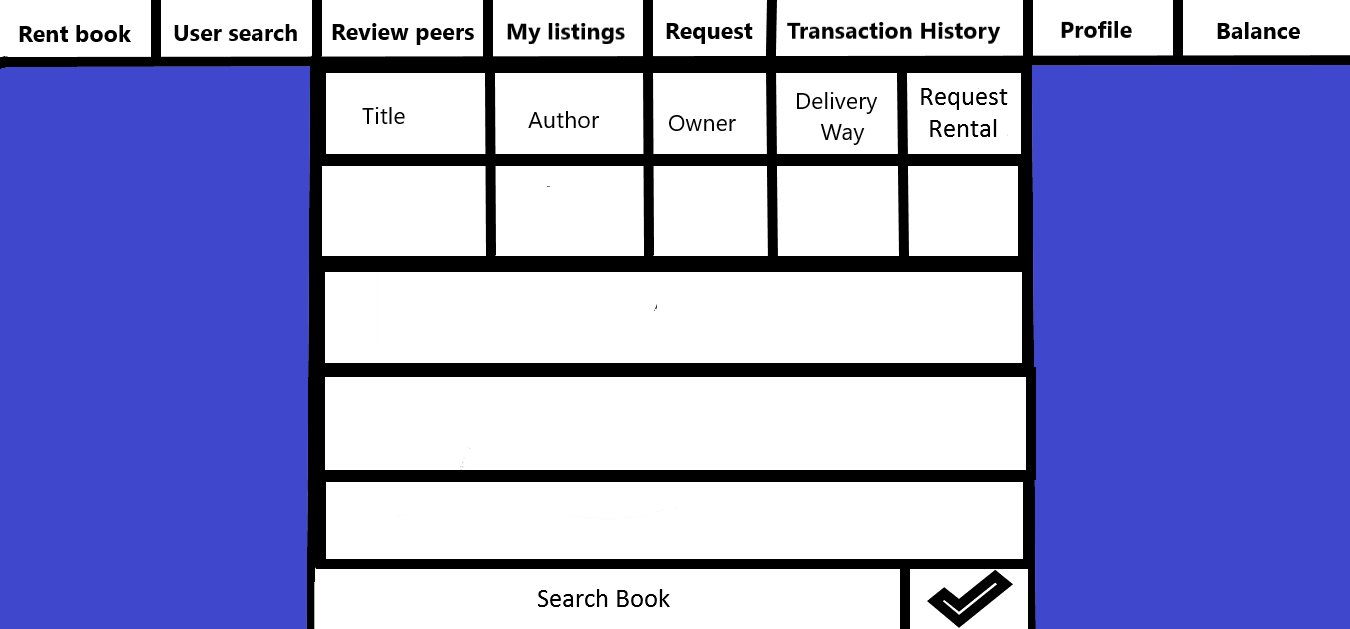
\includegraphics[width=\textwidth]{Mockup Screens/Rent Book.png}}
	\caption{Οθόνη "Rent Book" λειτουργικότητας}
	\label{Οθόνη "Rent Book" λειτουργικότητας}
\end{figure}

Η οθόνη αυτή περιέχει έναν πίνακα με στήλες με τίτλους "Title", "Author", "Owner", "Delivery Way" και ένα κουμπί "Request Rental". 

Η λειτουργικότητα του "Request Rental" είναι αυτή που εξηγείται ως "αίτηση ενοικίασης" στο κεφάλαιο \ref{Περιγραφή}.

Τα κελιά του πίνακα στη τελική έκδοση θα περιέχουν όλα τα διαθέσιμα βιβλία και τις πληροφορίες τους ανά στήλη, μαζί με την τιμή ενοικίασης ανά ημέρα (κάτω από το "Request Rental").

Επίσης υπάρχει και λειτουργία αναζήτησης συγκεκριμένου βιβλίου στο κάτω μέρος της οθόνης.

\subsection{User Search}

Στο Σχήμα \ref{Οθόνη "User Search" λειτουργικότητας} παρουσιάζεται mock-up οθόνη της λειτουργικότητας της αναζήτησης χρηστών.

\begin{figure}[H]
	\makebox[\textwidth]{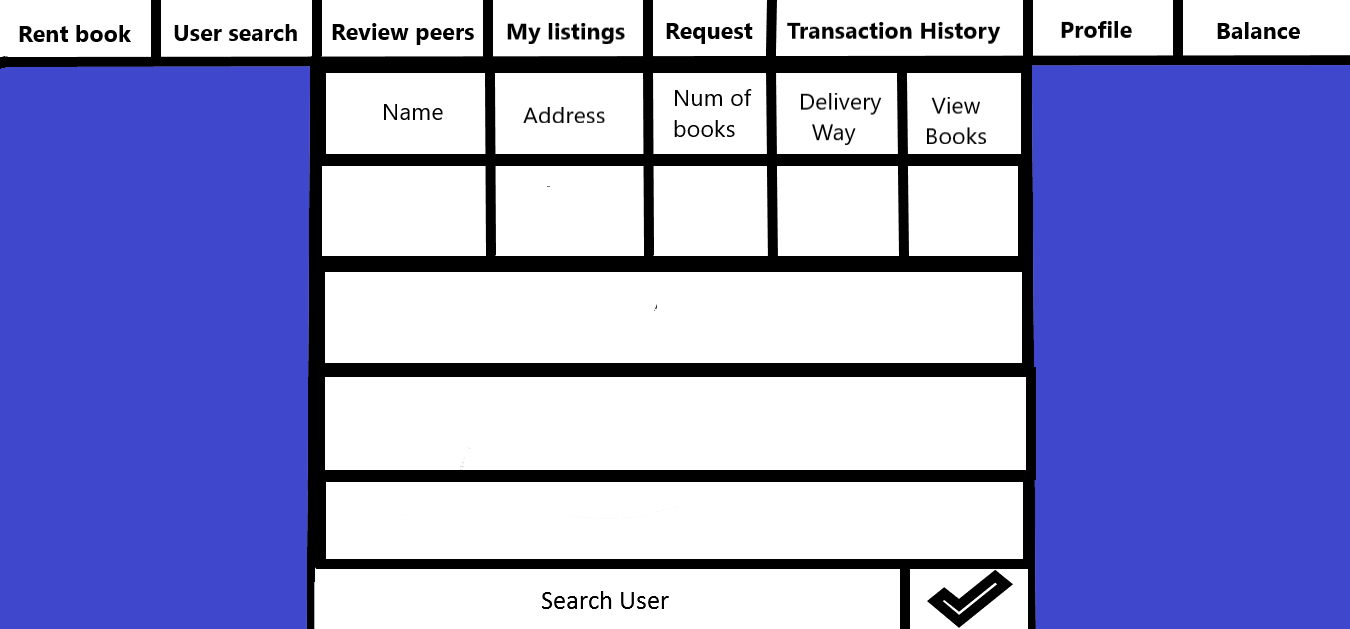
\includegraphics[width=\textwidth]{Mockup Screens/User Search.png}}
	\caption{Οθόνη "User Search" λειτουργικότητας}
	\label{Οθόνη "User Search" λειτουργικότητας}
\end{figure}

Παρατηρούμε ότι η οθόνη αυτή περιέχει έναν πίνακα με στήλες με τίτλους "Name", "Address", "Num of Books" "Delivery Way" και ένα κουμπί "View Books". 

Το κουμπί "View Books" μεταβιβάζει τον χρήστη σε μια σελίδα όπως τη σελίδα του "Rent Book" (Σχήμα \ref{Οθόνη "Rent Book" λειτουργικότητας} που θα περιέχει μόνο τα βιβλία του χρήστη που επιλέχθηκε.

Τα κελιά του πίνακα στη τελική έκδοση θα περιέχουν όλους τους χρήστες που πληρούν την αναζήτηση και τις πληροφορίες τους ανά στήλη.

Επίσης υπάρχει και λειτουργία αναζήτησης συγκεκριμένου χρήστη στο κάτω μέρος της οθόνης.

\subsection{Review Peers}

Στο Σχήμα \ref{Οθόνη "Review peers" λειτουργικότητας} παρουσιάζεται mock-up οθόνη της λειτουργικότητας του Review άλλων χρηστών.

\begin{figure}[H]
	\makebox[\textwidth]{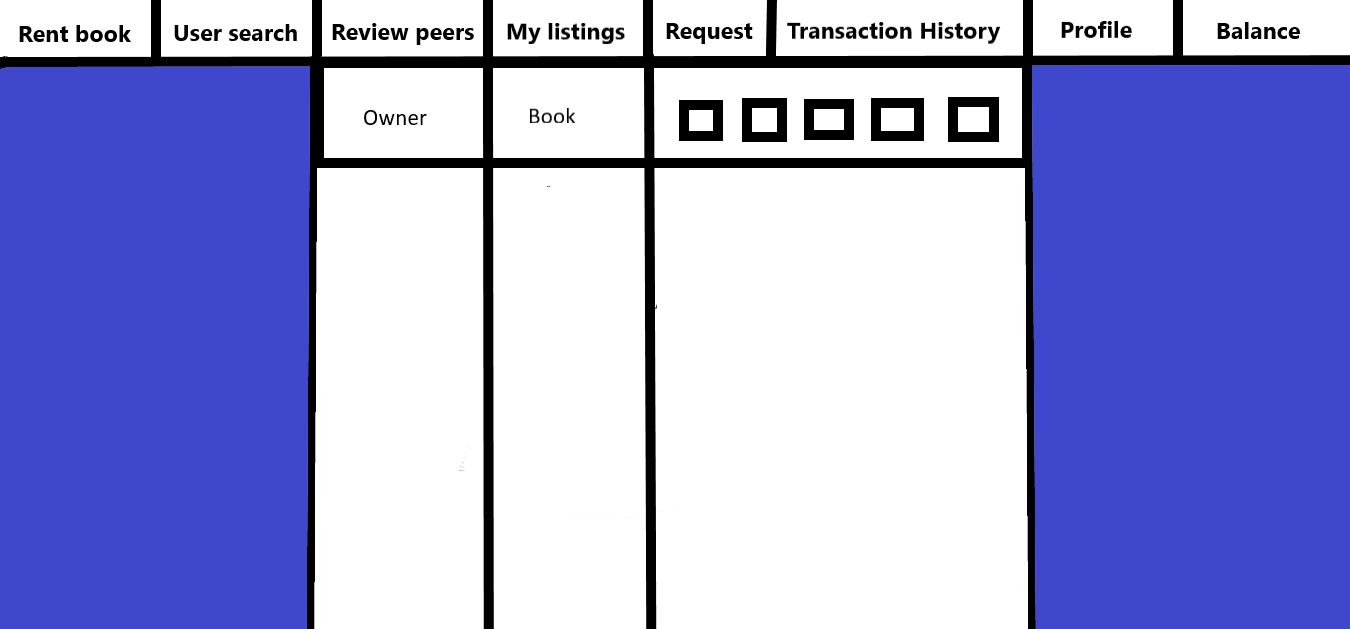
\includegraphics[width=\textwidth]{Mockup Screens/Review Peers.png}}
	\caption{Οθόνη "Review peers" λειτουργικότητας}
	\label{Οθόνη "Review peers" λειτουργικότητας}
\end{figure}

Παρατηρούμε ότι η οθόνη αυτή περιέχει έναν πίνακα με στήλες με τα ονόματα των χρηστών με τους οποίους έχουν γίνει προηγούμενες συναλλαγές, και το βιβλίο που ενοικιάστηκε.

Επίσης φαίνεται και ένα γραφικό δίπλα σε κάθε συναλλαγή με λειτουργικότητα της κριτικής του άλλου χρήστη από 1 έως 5 "αστεράκια".

Τα κελιά του πίνακα στη τελική έκδοση θα περιέχουν όλους τους χρήστες και τα βιβλία για τις προηγούμενες συναλλαγές που έχουν γίνει.

\subsection{My Listings}

Στο Σχήμα \ref{Οθόνη "My Listings" λειτουργικότητας} παρουσιάζεται mock-up οθόνη της λειτουργικότητας της προβολής των βιβλίων που προσφέρει ο χρήστης σε άλλους να νοικιάσουν, μαζί με δυνατότητα προσθήκης και αφαίρεσης άλλων βιβλίων.

\begin{figure}[H]
	\makebox[\textwidth]{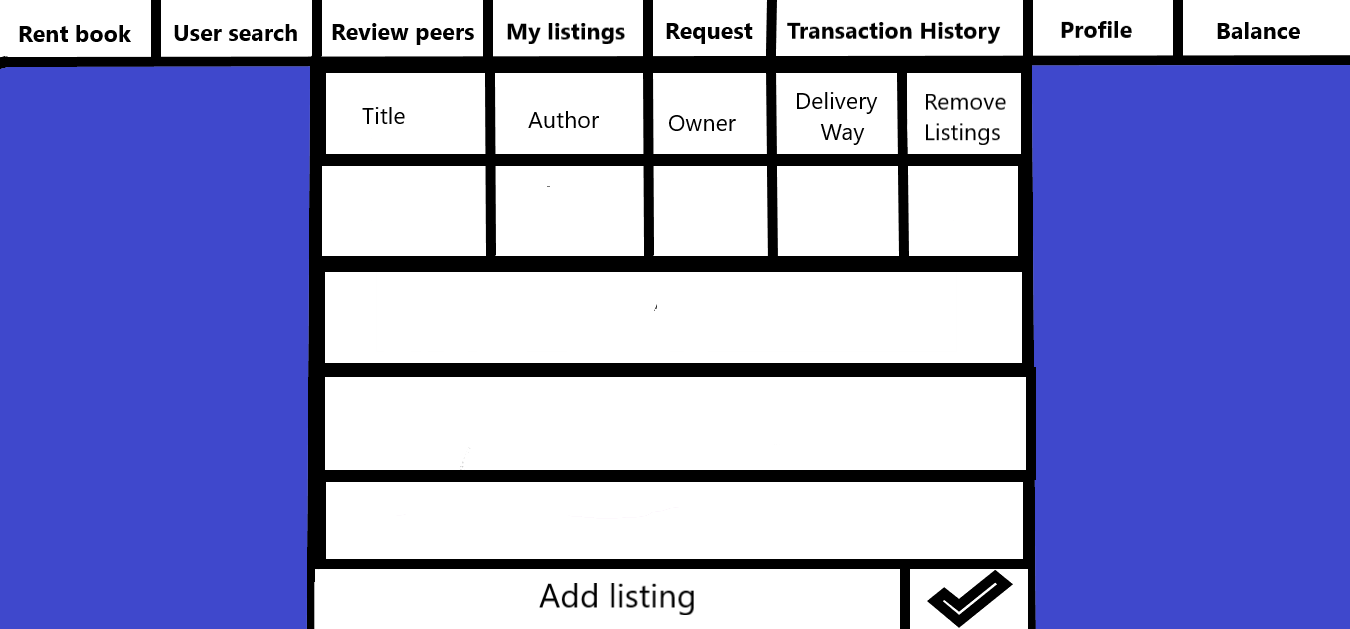
\includegraphics[width=\textwidth]{Mockup Screens/My Listings.png}}
	\caption{Οθόνη "My Listings" λειτουργικότητας}
	\label{Οθόνη "My Listings" λειτουργικότητας}
\end{figure}

Παρατηρούμε ότι η οθόνη αυτή περιέχει έναν πίνακα με στήλες με τίτλους "Title", "Author", "Owner", "Delivery Way" και κουμπιά "Remove Listing" και στο τέλος της σελίδας ένα κουμπί "Add Listing", όπου πλέον ο χρήστης συμπληρώνει τα στοιχεία του βιβλίου που θα νοικιάσει σε ένα popup screen.

Τα κελιά του πίνακα στη τελική έκδοση θα περιέχουν το σύνολο των βιβλίων που προσφέρει ο συνδεδεμένος χρήστης για ενοικίαση από άλλους.

\subsection{Requests}

Στο Σχήμα \ref{Οθόνη "Requests" λειτουργικότητας} παρουσιάζεται mock-up οθόνη της λειτουργικότητας της προβολής αιτήσεων άλλων και της αποδοχή τους (δηλαδή προσφοράς του βιβλίου στον χρήστη που το ζητάει και έκανε την αίτηση και αποδοχή του χρηματικού αντίτιμου). Επίσης στο κάτω μέρος της σελίδας υπάρχει ένα κουμπί που προσφέρει λειτουργικότητα δημιουργίας νέας αίτησης.

\begin{figure}[H]
	\makebox[\textwidth]{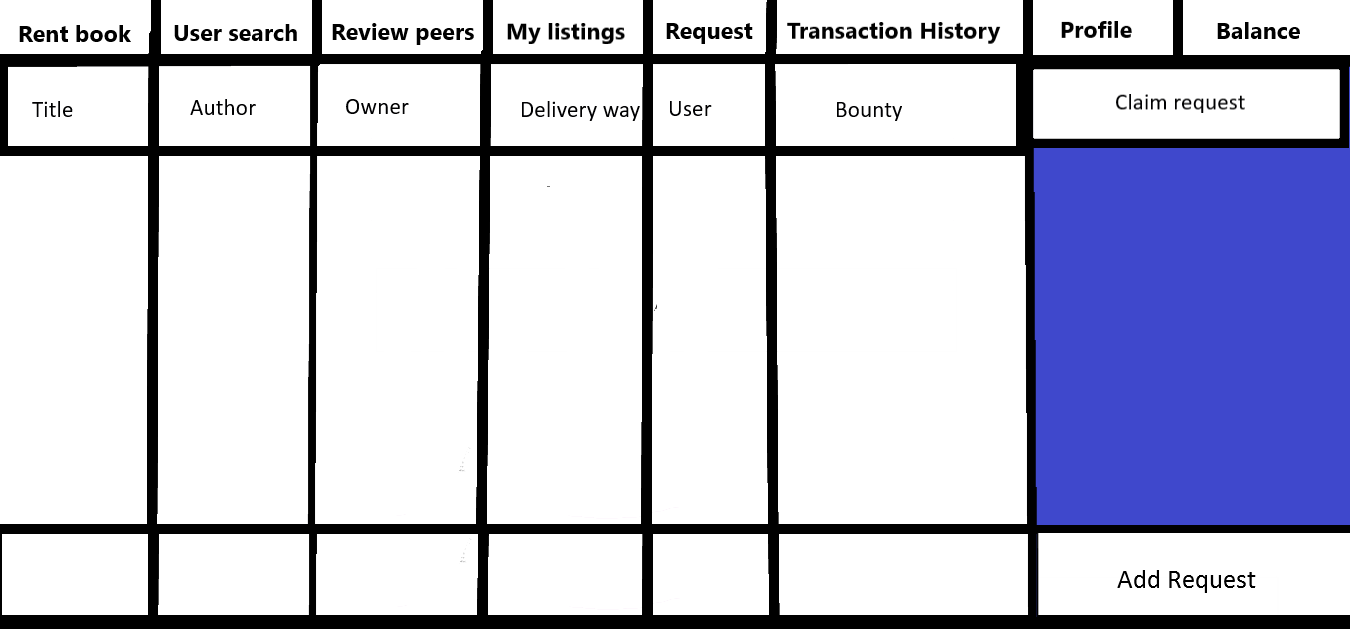
\includegraphics[width=\textwidth]{Mockup Screens/Request.png}}
	\caption{Οθόνη "Requests" λειτουργικότητας}
	\label{Οθόνη "Requests" λειτουργικότητας}
\end{figure}

Παρατηρούμε ότι η οθόνη αυτή περιέχει έναν πίνακα με στήλες με τίτλους "Title", "Author", "Owner", "Delivery Way", "User", "Bounty" και κουμπιά "Claim Request" και στο τέλος της σελίδας το κουμπί "Add Requests", όπου πλέον ο χρήστης συμπληρώνει τα στοιχεία του βιβλίου που ζητάει να νοικιάσει σε ένα popup screen.

Τα κελιά του πίνακα στη τελική έκδοση θα περιέχουν το σύνολο των στοιχείων για τα requests που είναι ενεργά εκείνη τη χρονική στιγμή.

\subsection{Transaction History}

Στο Σχήμα \ref{Οθόνη "Transaction History" λειτουργικότητας} παρουσιάζεται mock-up οθόνη της λειτουργικότητας της προβολής συναλλαγών (προηγούμενων και τρεχόντων) καθώς και της αποδοχής ή απόρριψης αιτημάτων και ανανέωσης κατάστασης κατοχής βιβλίου (δηλαδή ανανεώνεται όταν έχει φτάσει το βιβλίο στον ενοικιαστή και πίσω στον ιδιοκτήτη).

\begin{figure}[H]
	\makebox[\textwidth]{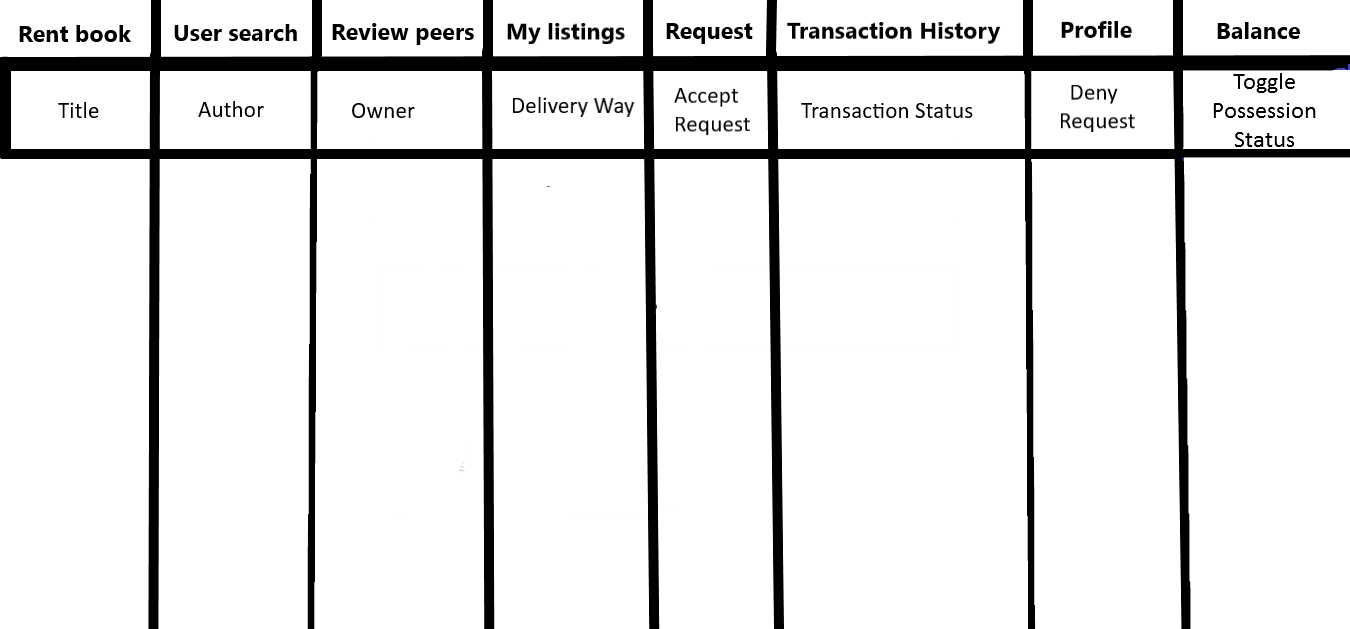
\includegraphics[width=\textwidth]{Mockup Screens/Transaction History.png}}
	\caption{Οθόνη "Transaction History" λειτουργικότητας}
	\label{Οθόνη "Transaction History" λειτουργικότητας}
\end{figure}

Παρατηρούμε ότι η οθόνη αυτή περιέχει έναν πίνακα με στήλες με τίτλους "Title", "Author", "Owner", "Delivery Way", "Transaction Status" και εναλλακτικά κουμπιά "Accept Request" και "Deny Request" ή "Toggle Possession Status" ή κανένα κουμπί, αντίστοιχα με την κατάσταση της συναλλαγής, όπως αναφέρεται στο κεφάλαιο \ref{Περιγραφή}.

Τα κελιά του πίνακα στη τελική έκδοση θα περιέχουν όλο το ιστορικό των συναλλαγών για τον χρήστη που είναι συνδεδεμένος.

\subsection{Profile}

Στο Σχήμα \ref{Οθόνη "Profile" λειτουργικότητας} παρουσιάζεται mock-up οθόνη της λειτουργικότητας της προβολής και αλλαγής των στοιχείων του λογαριασμού του συνδεδεμένου χρήστη.

\begin{figure}[H]
	\makebox[\textwidth]{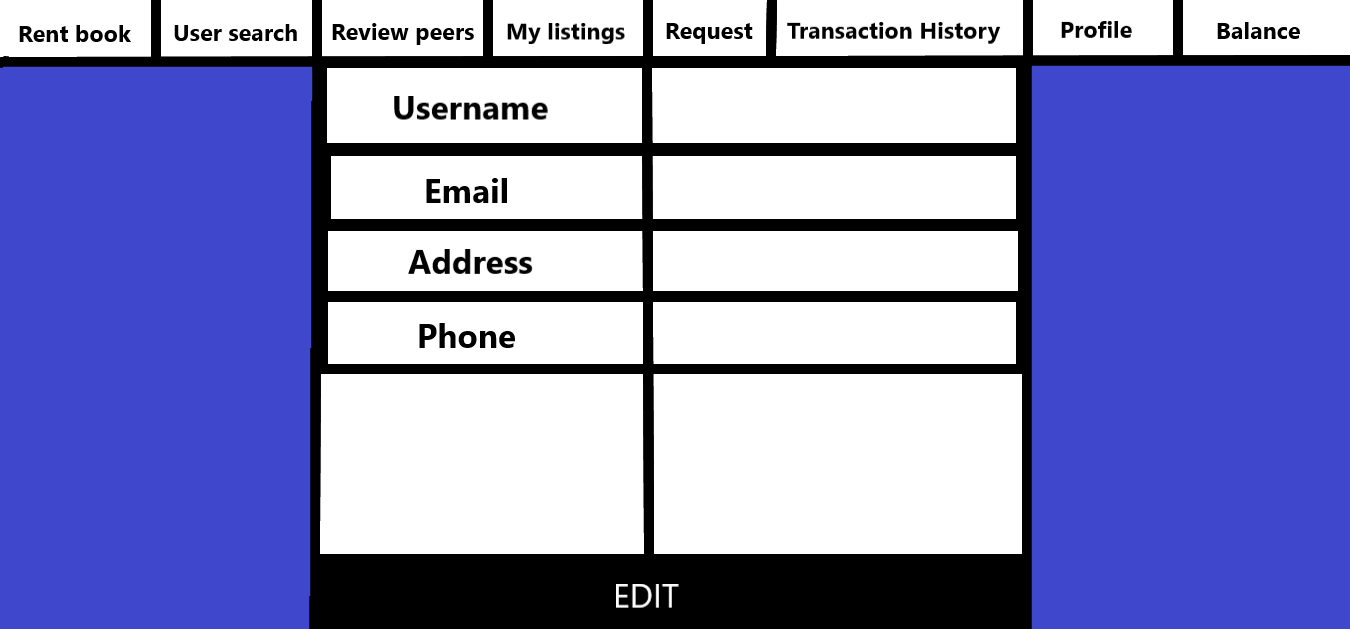
\includegraphics[width=\textwidth]{Mockup Screens/Profile.png}}
	\caption{Οθόνη "Profile" λειτουργικότητας}
	\label{Οθόνη "Profile" λειτουργικότητας}
\end{figure}

Παρατηρούμε ότι η οθόνη αυτή περιέχει έναν πίνακα με γραμμές με τίτλους "Username", "Email", "Address" και "Phone". Στη δεξιά μεριά του πίνακα προβάλλονται κάθε φορά τα στοιχεία του χρήστη.

Στη κάτω μεριά της οθόνης υπάρχει ένα κουμπί "Edit" το οποίο επιτρέπει στον χρήστη να ανανεώσει τα στοιχεία του.

\subsection{Balance}

Στο Σχήμα \ref{Οθόνη "Balance" λειτουργικότητας} παρουσιάζεται mock-up οθόνη της λειτουργικότητας της προβολής χρημάτων στον λογαριασμό και της προσθήκης και αφαίρεσης χρηματικού ποσού από τον λογαριασμό.

\begin{figure}[H]
	\makebox[\textwidth]{
\includegraphics[width=\textwidth]{Mockup Screens/Balance.png}}
	\caption{Οθόνη "Balance" λειτουργικότητας}
	\label{Οθόνη "Balance" λειτουργικότητας}
\end{figure}

Παρατηρούμε ότι η οθόνη αυτή περιέχει κουμπιά "Add Money" και "Remove Balance" για την προσθήκη και αφαίρεση χρηματικού ποσού από τον λογαριασμό αντίστοιχα.

Στη μέση της οθόνης υπάρχει ένα πεδίο "Balance" στο οποίο φαίνεται το ποσό που έχει διαθέσιμο ο χρήστης στον λογαριασμό του (έχουν αφαιρεθεί οι προκαταβολές και οι ανταμοιβές για αιτήσεις, τα οποία όμως μπορούν να επιστραφούν στο μέλλον).

\section{Συμμετοχή και Ρόλοι στη Συγγραφή του Κειμένου}

\begin{enumerate}
	\item \textbf{Γρηγόρης Καπαδούκας:} Author
	\item \textbf{Χρήστος Μπεστητζάνος:} Editor, Contributor
	\item \textbf{Νικόλαος Αυγέρης:} Peer Reviewer
	\item \textbf{Περικλής Κοροντζής:} Peer Reviewer
\end{enumerate}

\end{document}
